\chapter{COHORT AND PERIOD LIFE EXPECTANCY USING THE TWO-POINTS GOMPERTZ-MAKEHAM FRAILTY DISTRIBUTION}
\label{sec:sixth}
We observed in chapter 4 that in the early part of the 20th century, there was a very large difference in life expectancy between Spain and Italy on one hand and Norway and Sweden on the other. Over the last decade, that inequality has decreased and the period data suggest that since the 80's women in Spain and Italy are living longer than those in Norway and Sweden. See Figure \ref{fig:periodLifeExpect all}. But the cohort data suggest that women in Scandinavia are still living longer. see Figures \ref{fig:Number years lost max years90} - \ref{fig:Number of years lost 1970}. In this chapter we will illustrate with the help of the two-point Gompertz-Makeham frailty model that women in Italy and Spain living longer than those in Norway and Sweden may just be an artifact.  


\section{Two-points frailty distribution for cohort} 

In the following, we will study hundred cohorts over a period of hundred years. We index the cohort by  $ k=1 ;\dotsc; 100 $.
We assume a two-points frailty distribution for cohort $k$ with a baseline death intensity of the Gompertz-Makeham form

\begin{equation}
    \alpha_{0k}(t) = a_{k} + b_{k}c_{k}^t
    \label{gompertz3}
\end{equation}
Assume that the frailty $Z_{k}$ for cohort $k$ can take two values $z_{1k}$ and $z_{2k}$ with probabilities $P(Z=z_{1k}) = \pi_{1k}$ and $ P(Z=z_{2k}) = \pi_{2k}$ ; ~~ $\pi_{1k} + \pi_{2k} = 1 $.
For the cohort $k$ it follows from (\ref{gompertz3}) that:


\begin{equation*}
         A_{0k}(t) = \int_{0}^{t} \alpha_{0k}(u)du 
                 = a_{k}t + \frac{b_{k}(c_{k}^t-1)}{\log(c_{k})}
 \end{equation*}
The population survival function for the cohort $k$ is given by:


\begin{equation}
  S_{k}(t) = \exp(-A_{0}(t) z_{1k})\pi_{1k} + \exp(-A_{0}(t) z_{2k})\pi_{2k}
\end{equation}
cf. (\ref{survival_kap5})
The corresponding population hazard is obtain from (\ref{deathIntensity population2}) and (\ref{deathIntensity population3})


\begin{equation}
      \mu_{k}(t) = W_{k}(t)z_{1k}\alpha_{0k}(t) + (1 - W_{k}(t))z_{2k}\alpha_{0k}(t)
    \label{deathIntensityPopulation3kap2}           
\end{equation}
where 


\begin{equation}
   W_{k}(t) = \frac{\pi_{1k}\exp(-A_{0k}(t)z_{1k})}{\pi_{1k}\exp(-A_{0k}(t)z_{1k}) + \pi_{2k}\exp(-A_{0k}(t)z_{2k}) }
   \label{deathIntensity population3kap6}
\end{equation}
Using that $ S_{0k}(t) = \exp(-A_{0k}(t)) $, the expected life length of the cohort $k$ up to a given age $a$ for two-point Gompertz-Makeham frailty model is then:


\begin{equation}
        E[T_{a}] = \pi_{1k}\int_{0}^{a} S_{0k}(u)^{z_{1k}}du + \pi_{2k}\int_{0}^{a} S_{0k}(u)^{z_{2k}}du 
\end{equation}
cf. (\ref{life_expect_kapitel6})


\section{Two-points frailty distribution for period} 

In order to compute period mortality for a period of 100 years, we need information that describe how the parameters of the two-point Gompertz-Makeham frailty model have (hypothetically!) developed over a period of 200 years (namely the 100 years we focus on and a period of 100 years before that). We index these 200 years by $p = -99, -98, \dots,0, \dots,100$.
As discussed in chapter 3 the period mortality for period $p$ and age $t$ corresponds to the cohort mortality at age $t$ for the cohort born in year $k = p-t $.
The period population hazard can therefore be obtain by:

\begin{equation}
    \mu^{(p)} (t) = \mu_{p-t}  (t)
\end{equation}
where $p$ is the period and $t = 0, 1, 2, \cdots , 100$ is the age.
Because of the difficulty to integrate the hazard function, an approximation can be given by:

\begin{equation}
    \int_{0}^{t} \mu^{(p)}(u) du \approx \sum\limits_{x=0}^{t-1} \mu^{(p)} (t)
\end{equation}
The population survival  function of the period is obtain by:
 
 \begin{equation}
     S^{(p)}(t) = \exp(-\int_{0}^{t} \mu^{(p)}(u)du )
 \end{equation}
and the life expectancy of the period can be obtain by:

\begin{equation}
    E^{(p)}[T] = \int_{0}^{\omega} S^{(p)}(t)dt \approx \sum\limits_{x=0}^{\omega -1} S^{(p)}(t) 
\end{equation}
where $\omega$ is the maximum possible age.


    
    

\section{Comparison of the period and cohort mortality using the two-points frailty distribution with the baseline death intensity of the Gompertz-Makeham}

The parameters choosen for the various cohorts in the two-points Gompertz-Makeham frailty model are described in table \ref{parameters_table}. Here country A corresponds to Norway and Sweden and country B to Italy and Spain.
Figure \ref{fig:hazard periodCohort and frailty} compares the population mortality for country A and B for three different cohorts ($ k = 1, 50, 100 $).
Cohort 1 is the oldest cohort and cohort 100 is the youngest cohort. The rates are on logarithmic scale.


\begin{table}[tbh]

\begin{center}
    \captionof{table}{Values of the parameters in the two-points Gompertz-Makeham frailty model for 200 cohorts (indexed as $ k= -99, -98, \cdots, 0, 1, 2, \cdots, 100$)}
    \label{parameters_table}
    \begin{tabular}{ | l | l |  p{5cm}|}
    \hline
    Parameters & Country A  & Country B \\ 
    \hline
    a &\multicolumn{1}{m{4cm}|}{Equal to 0.005 for all  $k=-99, -98, \cdots, 0$.  Then decreasing exponentially to $3.10^{-5}$ for $k = 100$}& \multicolumn{1}{m{4cm}|}{ Equal to $0.010$ for all $k=-99, -98,\cdots, 0$. Then decreasing exponentially to $3.10^{-5}$ for  $k = 100$} \\ 
    \hline
    b &\multicolumn{1}{m{4cm}|}{Equal to $2.10^{-5}$ for all $k=-99, -98, \cdots, 0$.  Then decreasing exponentially to $10^{-5}$ for $k = 100$}& Same as for country A. \\ 
    \hline
    c & \multicolumn{1}{m{4cm}|}{Equal to 1.100 for all $k=-99, -98, \cdots, 100$.} & \multicolumn{1}{m{4cm}|}{ Equal to 1.098 for all $k=-99, -98,\cdots, 0$. Then increasing exponentially to 1.100 for  $k = 100$} \\  
    \hline
    $\pi_{1}$ &\multicolumn{1}{m{4cm}|}{Equal to 0.50 for all $k=-99, -98, \cdots, 100$.}& Same as for country A.\\  
    \hline
    $z_{1}$  &\multicolumn{1}{m{4cm}|}{Equal to 0.50 for all $k=-99, -98, \cdots, 100$.}& \multicolumn{1}{m{4cm}|}{ Equal to $0.40$ for all $k=-99,-98, \cdots, 0$. Then increasing linearly to 0.50 for  $k = 50$ and staying at that value until $k = 100$} \\ 
    \hline
    $z_{2}$ &\multicolumn{1}{m{4cm}|}{Equal to 2 for all $k=-99, -98, \cdots, 100$.}& \multicolumn{1}{m{4cm}|}{ Equal to 3 for all $k=-99, -98,\cdots, 0$. Then decreasing linearly to 2 for  $k = 50$ and staying at that value until $k = 100$} \\ 
    \hline
    \end{tabular}
\end{center}

\end{table}



   \begin{figure}[tbh]
             \centering
              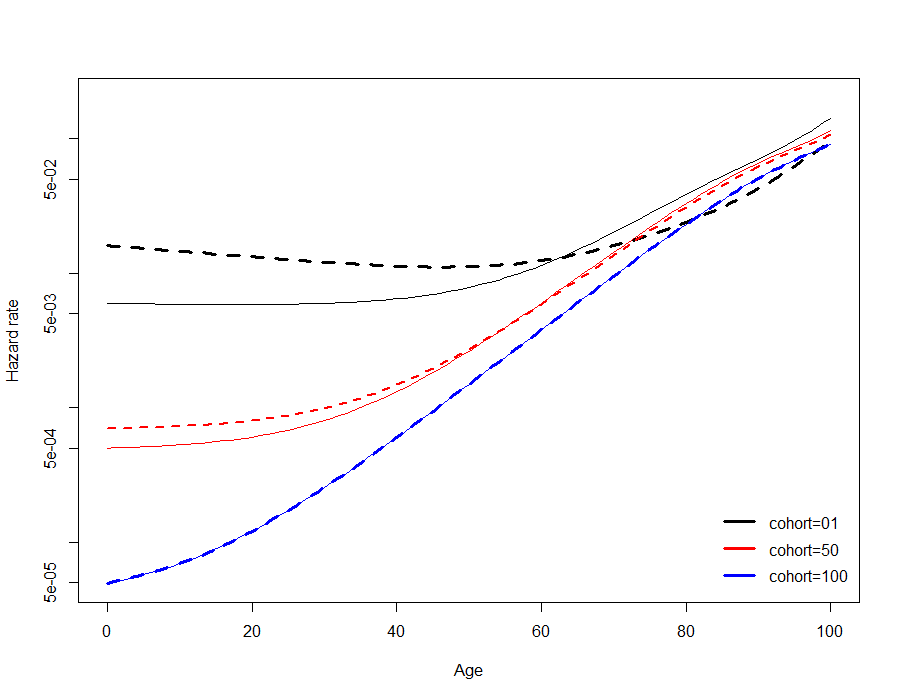
\includegraphics[ width=0.8\linewidth]{figures/Period_Cohort_mort_A_B.png}
              \caption{Population mortality for the two points Gompertz - Makeham frailty model for three cohorts (k= 01, 50, 100) for country A (drawn line) and country B (dashed line)}
              \label{fig:hazard periodCohort and frailty}
    \end{figure}



For cohort 1, we observe a huge difference of mortality rates between country A and country B among the younger ages.
That is due to higher number of frail individuals in country B than in country A. The mortality rates are therefore lower in country A than in country B.  
After the age of 60 years, we observe that the number of frail individuals have steadily decreased resulting in country B having lower mortality rates than country A.   


For cohort  50, we observe that the mortality rates are greater in country B than in country A from birth until the age of 45 years. Beyond the age of 45 years, country A and country B have about the same mortality rates (solid and dotted red lines). The overlap of mortality in country A and country B after the age of 45 year is mainly due to the fact that frail individuals in country B will tend to die first and those remaining will have the same frailty level as individuals in country A.

Finally we observe that in cohort 100, there is no difference in mortality in country A and country B (solid and dotted blue lines). 

% (\cite{VM04}) bruke den hvor jeg sammeligner landene




  \begin{figure}[tbh]
             \centering
              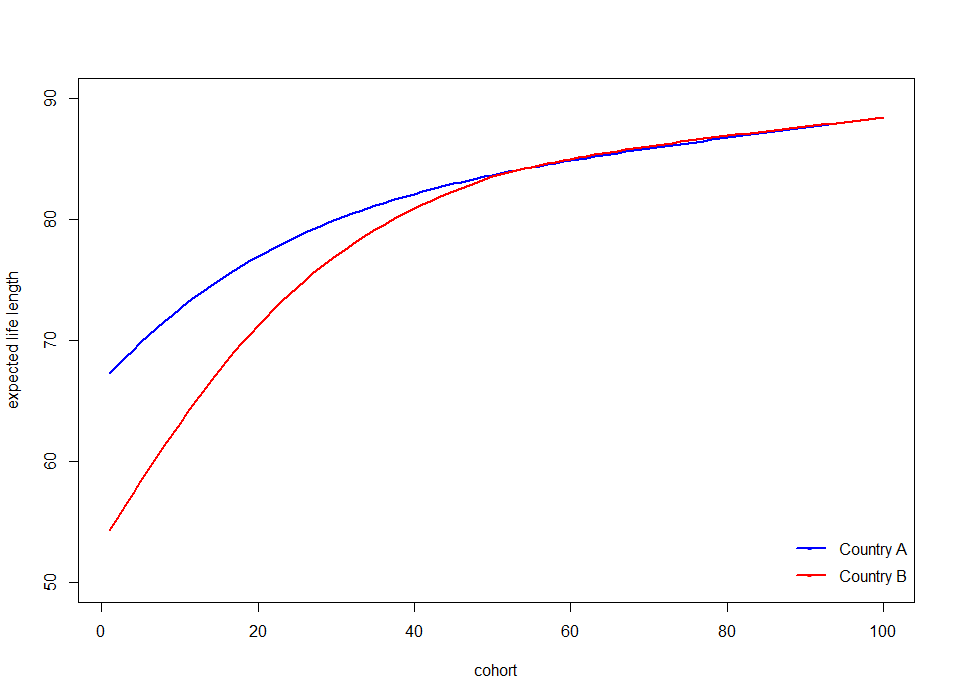
\includegraphics[ width=0.8\linewidth]{figures/Cohort_life_expect_A_B.png}
              \caption{Cohort life expectancy illustrating country A and country B.}
              \label{fig:Life expectCohortAB and frailty}
    \end{figure}
    


Figure \ref{fig:Life expectCohortAB and frailty} shows the cohort life expectancy in country A in blue and country B in red. We observe that country A has the highest life expectancy back in time. But for the younger cohorts the life expectancy in country B increases and attains the same level of life expectancy as in country A. 




   \begin{figure}[tbh]
             \centering
              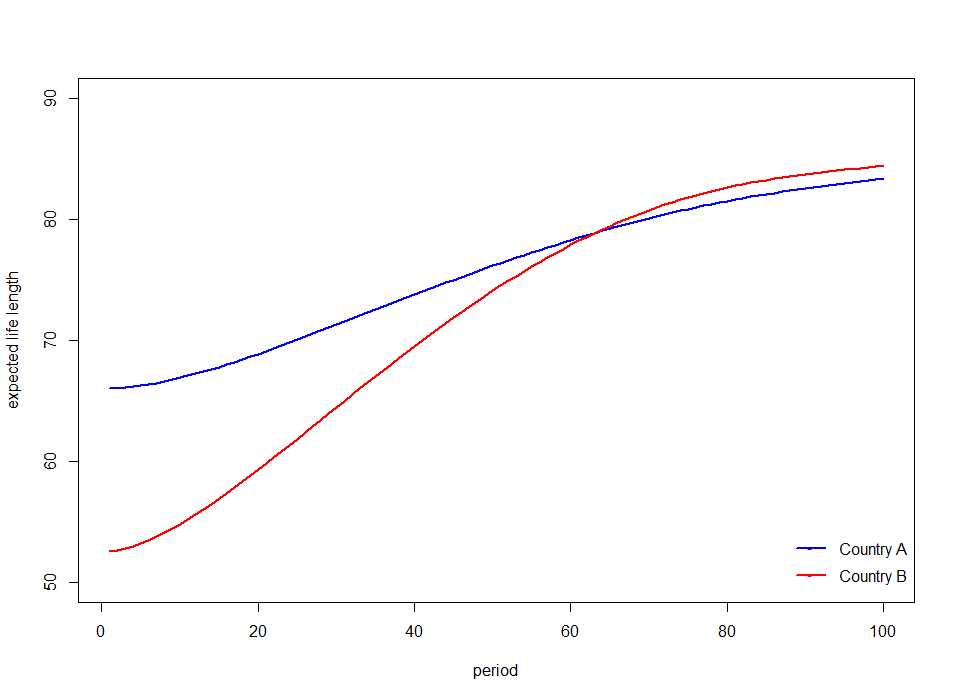
\includegraphics[ width=0.8\linewidth]{figures/Period_life_expect_A_B.png}
              \caption{Period life expectancy illustrating country A and country B.}
              \label{fig: Life expectPeriodAB and frailty}
    \end{figure}


In figure \ref{fig: Life expectPeriodAB and frailty} we have an illustration of the  period life expectancy in country A and country B. We observe that country A has the highest life expectancy during the earlier period. But the improvement of mortality in country B result in a rapid increase of life expectancy. This will result in the cross over we observed in the figure, where country B have higher life expectancy than country A for the most recent periods.


Based on the empirical study we had in the earlier chapter and the illustrative result we observed in this chapter, we can conclude that what we observed on Figure \ref{fig:periodLifeExpect all} in chapter 4 may be due to a selection effect and may therefore be an artifact. Since the 18th century, life expectancy have been higher in Norway and Sweden than Italy and Spain, and that trend still continue despite the significant reduction of the expected life length gap between countries in the Mediterranean and those in Scandinavia.


%https://www.ncbi.nlm.nih.gov/pmc/articles/PMC5191885/















 





